\chapter{Diagrammes d'architecture}

Cette section contient les diagrammes d'architecture du projet. Cette section est divisée en deux parties, la première se concentre sur le site web tendit que la seconde se concentre sur le web service qui sera utilisée par les terminaux mobiles.
 
\newpage
\section{Le site web}

\begin{figure}[H]
	\begin{center}\fbox{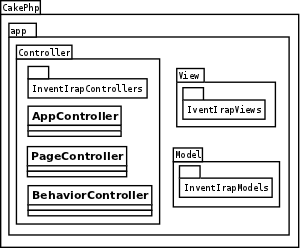
\includegraphics[]{images/architecture.png}}\end{center}
	\caption{Architecture générale du projet}
\end{figure}

Voici l'architecture générale du projet. Cakephp contient un dossier app qui contient principalement trois dossiers : Controller, View et Model. 

Le dossier View va contenir, entre autre, les classes "views" décrites dans le chapitre précédent. Le dossier Model va contenir, entre autre, les classes "models" décrites dans le chapitre précédent. Ces dossiers contiennent aussi d'autres sous dossiers propre à cakephp pour que celui-ci puisse fonctionner correctement.


Et enfin, le dossier Controller va contenir, en plus des classes "controllers" du chapitre précédent, deux autres classes : AppController et PageController. Ce sont des classes utiles au fonctionnement de cakephp, nous n'avons pas à les modifier.

\section{Le web service}
Les deux applications mobiles (Android et iOS) utiliseront la bibliothèque XZing \footnote{Lien vers le site web : \href{http://code.google.com/p/zxing/}{http://code.google.com/p/zxing/}} sous licence Apache 2.0.
Cette biliothèque permet de décoder un QRCode à partir d'une photo prise depuis un smartphone.

Pour l'interaction entre l'application et les terminaux mobiles, nous utiliserons la fonctionnalité de CakePHP pour créer des webservices capables de gérer un flux de données sous forme XML.
L'application contiendra donc un controleur qui servira des requêtes demandant des informations sur identifiant de matériel.

\begin{figure}[H]
	\begin{center}\fbox{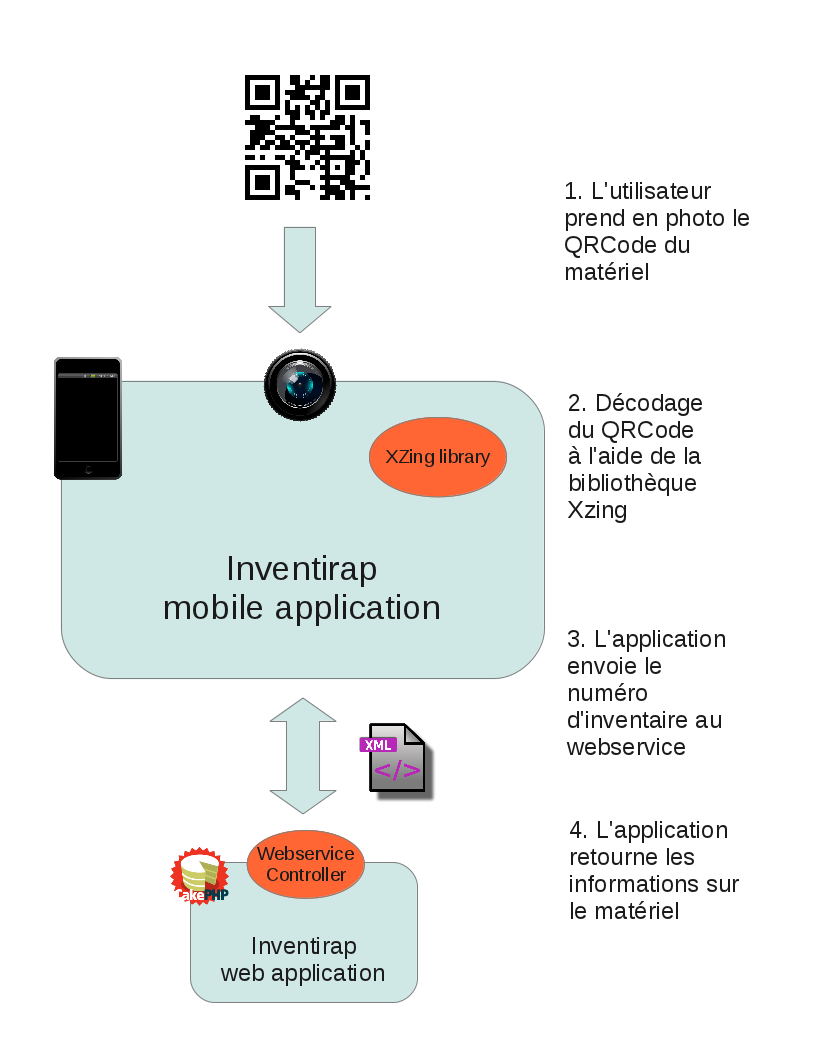
\includegraphics[scale=0.75]{images/webservice_schema.png}}\end{center}
	\caption{Schéma générale du webservice}
\end{figure}

\begin{figure}[H]
	\begin{center}\fbox{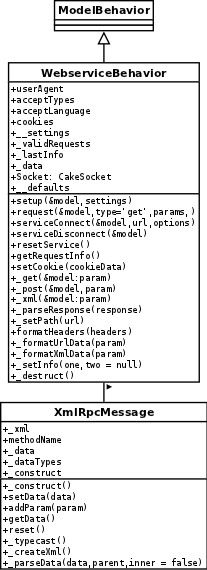
\includegraphics[]{images/webserviceController.png}}\end{center}
	\caption{Description des classes utiles au webservice}
\end{figure}

La classe WebserviceBehavior sert de contrôleur principale pour gérer les requêtes des terminaux mobiles. La classe WmlRpcMessage représente ces requête du côte du serveur pour cakephp.
